% This is samplepaper.tex, a sample chapter demonstrating the
% LLNCS macro package for Springer Computer Science proceedings;
% Version 2.21 of 2022/01/12
%
\documentclass[runningheads]{llncs}
%
\usepackage[T1]{fontenc}
% T1 fonts will be used to generate the final print and online PDFs,
% so please use T1 fonts in your manuscript whenever possible.
% Other font encondings may result in incorrect characters.
%
\usepackage{graphicx}
% Used for displaying a sample figure. If possible, figure files should
% be included in EPS format.
%
% If you use the hyperref package, please uncomment the following two lines
% to display URLs in blue roman font according to Springer's eBook style:
%\usepackage{color}
%\renewcommand\UrlFont{\color{blue}\rmfamily}
%\urlstyle{rm}
%


% \usepackage{setspace}
%\AtBeginDocument{\setstretch{.9}}
%\doublespacing  % doublespacing is done after title and before abstract

\usepackage{caption}
\usepackage{subcaption}
\usepackage[title]{appendix}

%\usepackage[margin=0.25in]{geometry}

%\usepackage{lineno}
%\linenumbers

% \usepackage{fullpage}
\usepackage{authblk}
\usepackage[utf8]{inputenc}
\usepackage{amsmath,bm}
\usepackage{amsthm}
\usepackage{amssymb}
\usepackage{hyperref}
\usepackage{adjustbox}
\usepackage{multirow}
\usepackage{graphicx}
\usepackage{booktabs}
\usepackage{caption}
\usepackage{subcaption}
\usepackage[table]{xcolor}
\usepackage{tabu}
\usepackage{subcaption}
\usepackage{longtable}
\usepackage{amssymb}
\usepackage{footnote}
\usepackage{hyperref}
\usepackage{multirow}
\usepackage{comment}
\usepackage{cite}
\usepackage{threeparttable}
\usepackage{makecell}
\usepackage{mathtools} % for multiline-multicase equation
\usepackage{float}
\usepackage{array}
\usepackage{tabularx} % in the preamble
\usepackage{tikz}
\usepackage{ulem}
\usepackage{algorithm2e}

\usepackage{tabularx}
\newcolumntype{Y}{>{\centering\arraybackslash}X}
\newcolumntype{C}[1]{>{\centering\arraybackslash}m{#1}}

\usepackage{xcolor}
\newcommand{\add}[1]{{\color{blue} #1}}
\newcommand{\addb}[1]{{\color{red} #1}}
\newcommand{\SR}[1]{{\color{red} #1}}
\newcommand{\methodname}{{\color{purple}Method\_Name~}}

% \newtheorem{theorem}{Theorem}[section]
% \newtheorem{corollary}{Corollary}[theorem]
% \newtheorem{lemma}[theorem]{Lemma}

% \renewcommand{\thetheorem}{\arabic{theorem}}  % to start numbering from 1

%\usepackage{booktabs, caption, makecell}
%\renewcommand\theadfont{\bfseries}
\usepackage{subfiles} % For subfiles
\usepackage{hyperref}
\usepackage[labelfont=bf]{caption}

\usepackage{xcolor}

\renewcommand\theadalign{bc}
\renewcommand\theadfont{\bfseries}
\renewcommand\theadgape{\Gape[4pt]}
\renewcommand\cellgape{\Gape[4pt]}

\makesavenoteenv{tabular}
\makesavenoteenv{table}

\hypersetup{
    urlcolor=blue,
}

\begin{document}

%
\newcommand{\quartet}[4]{
  \begin{tikzpicture}
    % Nodes
    \node (a) at (0, 2) {};
    \node (b) at (0, 0) {};
    \node (c) at (3, 2) {};
    \node (d) at (3, 0) {};
    \node (center1) at (1, 1) {};
    \node (center2) at (2, 1) {};
    \node (name) at (1.5, -0.5) {$#1#2|#3#4$};

    % Edges
    \draw[thick] (a) -- (center1);
    \draw[thick] (b) -- (center1);
    \draw[thick] (center1) -- (center2);
    \draw[thick] (center2) -- (c);
    \draw[thick] (center2) -- (d);

    % Dots at nodes
    \fill (a) circle (2pt);
    \fill (b) circle (2pt);
    \fill (c) circle (2pt);
    \fill (d) circle (2pt);
    \fill (center1) circle (2pt);
    \fill (center2) circle (2pt);

    % Labels
    \node at (-0.2, 2) {#1};
    \node at (3.2, 2) {#3};
    \node at (3.2, 0) {#4};
    \node at (-0.2, 0) {#2};
  \end{tikzpicture}
}

\newcommand{\fivetax}[5]{
\begin{tikzpicture}
% Nodes
\node (a) at (0, 2) {};
\node (b) at (0, 0) {};
\node (c) at (3, 2) {};
\node (d) at (3, 0) {};
\node (x) at (0.5, 1.5) {};
\node (e) at (0, 1) {};

\node (center1) at (1, 1) {};
\node (center2) at (2, 1) {};

% Edges
\draw[thick] (a) -- (x);
\draw[thick] (center1) -- (x);
\draw[thick] (b) -- (center1);
\draw[thick] (center1) -- (center2);
\draw[thick] (center2) -- (c);
\draw[thick] (center2) -- (d);
\draw[thick] (e) -- (x);

% Dots at nodes
\fill (a) circle (2pt);
\fill (b) circle (2pt);
\fill (c) circle (2pt);
\fill (d) circle (2pt);
\fill (x) circle (2pt);
\fill (e) circle (2pt);
\fill (center1) circle (2pt);
\fill (center2) circle (2pt);

% Labels
\node at (-0.2, 2) {#1};
\node at (3.2, 2) {#3};
\node at (3.2, 0) {#4};
\node at (-0.2, 0) {#2};
\node at (-0.2, 1) {#5};
\end{tikzpicture}
}

\newcommand{\fivetaxcol}[5]{
\begin{tikzpicture}
% Nodes
\node (a) at (0, 2) {};
\node (b) at (0, 0) {};
\node (c) at (3, 2) {};
\node (d) at (3, 0) {};
\node (x) at (0.5, 1.5) {};
\node (e) at (0, 1) {};

\node (center1) at (1, 1) {};
\node (center2) at (2, 1) {};

% Edges
\draw[thick] (a) -- (x);
\draw[thick] (center1) -- (x);
\draw[thick] (b) -- (center1);
\draw[thick] (center1) -- (center2);
\draw[thick] (center2) -- (c);
\draw[thick] (center2) -- (d);
\draw[thick, red] (e) -- (x);


% Dots at nodes
\fill (a) circle (2pt);
\fill (b) circle (2pt);
\fill (c) circle (2pt);
\fill (d) circle (2pt);
\fill (x) circle (2pt);
% \fill[red] (e) circle (2pt);
\fill (e) circle (2pt);
\fill (center1) circle (2pt);
\fill (center2) circle (2pt);

% Labels
\node at (-0.2, 2) {#1};
\node at (3.2, 2) {#3};
\node at (3.2, 0) {#4};
\node at (-0.2, 0) {#2};
\node at (-0.2, 1) {#5};
\end{tikzpicture}
}

\newcommand{\fivetaxinv}[5]{
\begin{tikzpicture}
% Nodes
\node (a) at (0, 2) {};
\node (b) at (0, 0) {};
\node (c) at (3, 2) {};
\node (d) at (3, 0) {};
\node (x) at (0.5, 0.5) {};
\node (e) at (0, 1) {};

\node (center1) at (1, 1) {};
\node (center2) at (2, 1) {};

% Edges
\draw[thick] (a) -- (center1);
\draw[thick] (center1) -- (x);
\draw[thick] (b) -- (x);
\draw[thick] (center1) -- (center2);
\draw[thick] (center2) -- (c);
\draw[thick] (center2) -- (d);
\draw[thick] (e) -- (x);

% Dots at nodes
\fill (a) circle (2pt);
\fill (b) circle (2pt);
\fill (c) circle (2pt);
\fill (d) circle (2pt);
\fill (x) circle (2pt);
\fill (e) circle (2pt);

\fill (center1) circle (2pt);
\fill (center2) circle (2pt);

% Labels
\node at (-0.2, 2) {#1};
\node at (3.2, 2) {#3};
\node at (3.2, 0) {#4};
\node at (-0.2, 0) {#2};
\node at (-0.2, 1) {#5};
\end{tikzpicture}
}

\newcommand{\fivetaxmult}[5]{
\begin{tikzpicture}
% Nodes
\node (a) at (0, 2) {};
\node (b) at (0, 0) {};
\node (c) at (3, 2) {};
\node (d) at (3, 0) {};
\node (x) at (2.5, 0.5) {};
\node (x2) at (2.5, 1.5) {};
\node (x3) at (1.5, 1) {};
\node (y) at (0.5, 1.5) {};
\node (e) at (3, 1) {};
\node (e2) at (2, 2) {};
\node (e3) at (1.5, 0) {};

\node (center1) at (1, 1) {};
\node (center2) at (2, 1) {};

% Edges
\draw[thick] (a) -- (center1);
\draw[thick] (center1) -- (b);
% \draw[thick] (b) -- (x);
\draw[thick] (center1) -- (center2);
\draw[thick] (center2) -- (c);
\draw[thick] (center2) -- (d);

\draw[thick, dotted, red, shorten <=-1mm, shorten >=-1mm] (e) -- (x);
\draw[thick, dotted, red, shorten <=-1mm, shorten >=-1mm] (e2) -- (x2);
\draw[thick, dotted, red, shorten <=-1mm, shorten >=-1mm] (e3) -- (x3);


% Dots at nodes
\fill (a) circle (2pt);
\fill (b) circle (2pt);
\fill (c) circle (2pt);
\fill (d) circle (2pt);
% \fill (x) circle (2pt);
\fill (e) circle (2pt);
\fill (e2) circle (2pt);
\fill (e3) circle (2pt);
\fill (center1) circle (2pt);
\fill (center2) circle (2pt);

% Labels
\node at (-0.2, 2) {#1};
\node at (3.2, 2) {#3};
\node at (3.2, 0) {#4};
\node at (-0.2, 0) {#2};
\node at (3.2, 1) {#5};
\node at (1.8, 2) {#5};
\node at (1.7, 0) {#5};
\end{tikzpicture}
}







\newcommand{\fivetaxdccol}[5]{
\begin{tikzpicture}
% Nodes
\node (a) at (0, 2) {};
\node (b) at (0, 0) {};
\node (c) at (3, 2) {};
\node (d) at (3, 0) {};
\node (x) at (2.5, 0.5) {};
\node (x2) at (2.5, 1.5) {};
\node (x3) at (1.5, 1) {};
\node (y) at (0.5, 1.5) {};
\node (e) at (3, 1) {};
\node (e2) at (2, 2) {};
\node (e3) at (1.5, 0) {};

\node (center1) at (1, 1) {};
\node (center2) at (2, 1) {};

% Edges
\draw[thick] (a) -- (center1);
\draw[thick] (center1) -- (b);
% \draw[thick] (b) -- (x);
\draw[thick] (center1) -- (center2);
\draw[thick] (center2) -- (c);
\draw[thick] (center2) -- (x);
\draw[thick] (x) -- (d);

\draw[thick, red] (e) -- (x);



% Dots at nodes
\fill (a) circle (2pt);
\fill (b) circle (2pt);
\fill (c) circle (2pt);
\fill (d) circle (2pt);
% \fill (x) circle (2pt);
% \fill[red] (e) circle (2pt);
\fill (e) circle (2pt);
\fill (center1) circle (2pt);
\fill (center2) circle (2pt);
\fill (x) circle (2pt);

% Labels
\node at (-0.2, 2) {#1};
\node at (3.2, 2) {#3};
\node at (3.2, 0) {#4};
\node at (-0.2, 0) {#2};
\node at (3.2, 1) {#5};
% \node at (1.8, 2) {#5};
% \node at (1.7, 0) {#5};
\end{tikzpicture}
}

\newcommand{\fivetaxdc}[5]{
\begin{tikzpicture}
% Nodes
\node (a) at (0, 2) {};
\node (b) at (0, 0) {};
\node (c) at (3, 2) {};
\node (d) at (3, 0) {};
\node (x) at (2.5, 0.5) {};
\node (x2) at (2.5, 1.5) {};
\node (x3) at (1.5, 1) {};
\node (y) at (0.5, 1.5) {};
\node (e) at (3, 1) {};
\node (e2) at (2, 2) {};
\node (e3) at (1.5, 0) {};

\node (center1) at (1, 1) {};
\node (center2) at (2, 1) {};

% Edges
\draw[thick] (a) -- (center1);
\draw[thick] (center1) -- (b);
% \draw[thick] (b) -- (x);
\draw[thick] (center1) -- (center2);
\draw[thick] (center2) -- (c);
\draw[thick] (center2) -- (x);
\draw[thick] (x) -- (d);

\draw[thick, shorten <=-1mm, shorten >=-1mm] (e) -- (x);



% Dots at nodes
\fill (a) circle (2pt);
\fill (b) circle (2pt);
\fill (c) circle (2pt);
\fill (d) circle (2pt);
% \fill (x) circle (2pt);
\fill (e) circle (2pt);
\fill (center1) circle (2pt);
\fill (center2) circle (2pt);
\fill (x) circle (2pt);

% Labels
\node at (-0.2, 2) {#1};
\node at (3.2, 2) {#3};
\node at (3.2, 0) {#4};
\node at (-0.2, 0) {#2};
\node at (3.2, 1) {#5};
% \node at (1.8, 2) {#5};
% \node at (1.7, 0) {#5};
\end{tikzpicture}
}


\newcommand{\triplet}[4]{
\begin{tikzpicture}
% Nodes
\node (a) at (0, 2) {};
\node (b) at (0, 0) {};
\node (center1) at (1, 1) {};
\node (c) at (2.5, 1) {};
\node (x) at (0.5, 0.5) {};
\node (y) at (0.5, 1.5) {};
\node (z) at (1.75, 1) {};
\node (d1) at (0, 1) {};
\node (d2) at (1, 2) {};
\node (d3) at (1.75, 0) {};

% Edges
\draw[thick] (a) -- (center1);
\draw[thick] (center1) -- (b);
\draw[thick] (center1) -- (c);

\draw[thick, dotted, red, shorten <=-1mm, shorten >=-1mm] (d1) -- (x);
\draw[thick, dotted, red, shorten <=-1mm, shorten >=-1mm] (d2) -- (y);
\draw[thick, dotted, red, shorten <=-1mm, shorten >=-1mm] (d3) -- (z);


% Dots at nodes
\fill (a) circle (2pt);
\fill (b) circle (2pt);
\fill (c) circle (2pt);
\fill (d1) circle (2pt);
\fill (d2) circle (2pt);
\fill (d3) circle (2pt);
\fill (center1) circle (2pt);

% Labels
\node at (-0.2, 2) {#1};
\node at (2.7, 1) {#3};
\node at (-0.2, 1) {#4};
\node at (1.2, 2) {#4};
\node at (1.95, 0) {#4};
\node at (-0.2, 0) {#2};
% \node at (3.2, 1) {#5};
% \node at (1.8, 2) {#5};
% \node at (1.7, 0) {#5};
\end{tikzpicture}
}


\newcommand{\linequart}[6]{
\begin{tikzpicture}
% Nodes
\node (a) at (0, 0) {};
\node (b) at (6, 0) {};
\node (cx) at (1.2, 0) {};
\node (xx) at (2.4, 0) {};
\node (dx) at (3.6, 0) {};
\node (yx) at (4.8, 0) {};

\node (c) at (1.2, 1) {};
\node (d) at (3.6, 1) {};
\node (x) at (2.4, -1) {};
\node (y) at (4.8, -1) {};

% Edges
\draw[thick] (a) -- (b);
\draw[dashed] (c) -- (cx);
\draw[dashed] (d) -- (dx);
\draw[dashed] (x) -- (xx);
\draw[dashed] (y) -- (yx);

% Dots at nodes
\fill (a) circle (2pt);
\fill (b) circle (2pt);
\fill (cx) circle (1.2pt);
\fill (dx) circle (1.2pt);
\fill (xx) circle (1.2pt);
\fill (yx) circle (1.2pt);
\fill (c) circle (1.5pt);
\fill (d) circle (1.5pt);
\fill (x) circle (1.5pt);
\fill (y) circle (1.5pt);

% Labels
\node at (-0.2, 0) {#1};
\node at (6.2, 0) {#2};
\node at (1, 1) {#3};
\node at (3.4, 1) {#4};
\node at (2.6, -1) {#5};
\node at (5, -1) {#6};

\end{tikzpicture}
}

\title{QT-WEAVER: Correcting quartet distribution improves phylogenomic analyses despite gene tree estimation error}
%
\titlerunning{QT-WEAVER}
% If the paper title is too long for the running head, you can set
% an abbreviated paper title here
%
\author{Navid Bin Hasan\inst{1,\dag}\orcidID{0009-0004-7792-9798} \and
Sohaib\inst{1,\dag}\orcidID{0009-0003-8861-4743} \and
Md. Shamsuzzoha Bayzid\inst{1}\orcidID{0000-0002-5640-0615}}
%
\authorrunning{N. Hasan et al.}
% First names are abbreviated in the running head.
% If there are more than two authors, 'et al.' is used.
%
\institute{\textsuperscript{1} Computer Science and Engineering, Bangladesh University of Engineering and Technology, Dhaka-1205, Bangladesh\\
\textsuperscript{\dag} These authors contributed equally to this work
\\
\email{navidhasan0@gmail.com, sohaibbinmusa@gmail.com, shams\_bayzid@cse.buet.ac.bd}}
%
\maketitle              % typeset the header of the contribution
%

\begin{abstract}
Summarizing individual gene trees into species phylogenies using coalescent-based methods has become a standard approach in phylogenomics. 
However, gene tree estimation error (GTEE) arising from a combination of reasons can potentially impact the accuracy of phylogenomic inference.
We, for the first time, introduce the problem of correcting the quartet distribution induced by a set of estimated gene trees, which involves updating the weights of the quartets to better reflect their relative importance within the gene tree distribution. We present QT-WEAVER, which learns the conflicts within the quartet distribution induced by a given set of gene trees and generates an updated quartet distribution by adjusting the weights accordingly. Experimental studies on a collection of simulated and empirical data sets suggest that QT-WEAVER can effectively account for GTEE, which results in a substantial improvement in the species tree accuracy. %Additionally, the concept of quartet conflicts and related algorithmic and combinatorial innovations introduced in this study will benefit various quartet-based computations. 
% Therefore, QT-WEAVER advances the state-of-the-art in species tree estimation from gene trees in the face of GTEE. 
% QT-WEAVER is freely available in open-source form at \url{https://github.com/navidh86/QT-WEAVER}. 
The full version of this paper is available at \url{https://www.biorxiv.org/content/10.1101/2024.11.11.622962}.

%quartets that is often closer to the quartet distribution of true gene trees than that of the estimated gene trees, and thereby accounting for gene tree estimation error.

%accuracy of species tree inference. 
%Remarkably, QT-GILD not only imputes the missing quartets but it can also account for gene tree estimation error.

%Remarkably, QT-GILD not only imputes the missing quartets but it can also ``correct’’ the estimated quartets -- resulting in a set of quartets that is often closer to the quartet distribution of true gene trees than that of the estimated gene trees, and thereby accounting for gene tree estimation error.  %QT-GILD -- with its auto-encoder based deep learning approach combined with concepts from NLP and the demonstrated notable improvements in tree accuracy -- significantly advances the state-of-the-art in species tree estimation from gene trees despite missing data. 


%Read this: https://academic.oup.com/mbe/article/37/5/1495/5685817?searchresult=1

%add model independence from this paper.

% needing no explicit modeling of the subject system and reasons for missing data

%Although there is a continuing effort to make models more realistic (Ronquist and Huelsenbeck 2003; Stamatakis 2014), model misspecification is and will likely be the norm rather than the exception.

%\keywords{Species tree, gene tree, incomplete lineage sorting (ILS), quartet distribution, quartet consistency, missing data, deep learning, autoencoder.}

\keywords{Species tree \and Gene tree \and Incomplete lineage sorting (ILS) \and Quartet distribution \and Quartet consistency.}
\end{abstract}


\vspace{-25pt}
\section{Introduction}
\vspace{-8pt}
Species tree estimation from multiple genes is commonly done through concatenation, which combines sequence alignments from different loci into a single supermatrix and then computes a tree on the supermatrix. While concatenation can produce accurate species trees when gene trees are concordant, it can be statistically inconsistent~\cite{roch2015likelihood,consensus-inconsistent}, and produce incorrect trees with high support~\cite{kubatko-degnan-2007} when gene trees differ from the species tree. As a result, summary methods~\cite{mpest,astral,larget-bioinf2010,glass,stem,svdquartet,steac,njst,wqfm,astrid,stelar} that combine estimated gene trees while accounting for gene tree discordance have drawn great interest. However, summary methods are prone to gene tree estimation errors (GTEE), which can arise from various reasons including short gene sequences, inaccurate alignments, and the limitations of the models and algorithms used for inferring gene trees from sequence data. 
As GTEE is a major contributor to inaccuracies of summary methods, there has been great interest in developing tools~\cite{notung,treefix,rasmussen2011bayesian,traction,profilenj,tt,treefix-dtl-bansal2015improved,nguyen2012accounting,jacox2017resolution,lafond2017gene} to account for GTEE for improved species tree estimations. However, most of these methods require an accurate reference tree, which itself can be hard to obtain due to GTEE. %Moreover, the more accurate Bayesian methods are not scalable to genome-level data.
% Most of these methods are species tree aware as they use a reference species tree in addition to the input gene trees. These species tree aware methods essentially reconcile/modify gene trees to make them closer in distance to the species tree by minimizing a species tree aware cost function. However, gene trees could be discordant and are not always expected to closely match the species tree. %such as Robinson Foulds distance,  inferred evolutionary events (GDL), etc., 
% %even when the true gene and species trees are discordant. 
% Additionally, ``integrative'' methods such as ProfileNJ~\cite{profilenj} and TreeFix~\cite{treefix} use available sequence data as well as the estimated gene trees and reference species trees. Obtaining a reasonably accurate reference species tree despite substantial amounts of GTEE is difficult and the inaccuracy in the reference tree may have cascading effects on gene tree corrections. More importantly, species tree aware methods, specifically TreeFix and TRACTION~\cite{traction}, have been criticized for their potential to increase GTEE where gene trees are discordant with species trees~\cite{zhiyan}. Bayesian techniques for co-estimating both gene trees and species trees such as BEST~\cite{best}, *BEAST~\cite{heled-drummond}, and PHYLDOG~\cite{boussau2013genome} 
% can produce substantially more accurate gene and species trees than other methods, but are not scalable to genome-level analyses~\cite{bayzid2013naive,smith2013target,bayzid-incomplete,leache-rannala,szollHosi2015inference}.
%Thus, despite significant attempts to account for GTEE, substantial challenges remain.\\
In this study, we address the problem of GTEE 
% in the context of species tree estimation
, by formulating the \textit{Quartet Distribution Correction} (QDC) problem, where we seek to ``correct'' the distribution of quartets induced by a given set of estimated gene trees. QDC attempts to account for GTEE without resorting to any reference species tree.
%Quartet-based summary methods have drawn considerable attention because of their ability to produce highly accurate species trees. ASTRAL, the most widely used summary method, infers a species tree by maximizing the number of quartets in the gene trees that are consistent with the species tree. Another class of methods (known as quartet amalgamation techniques, such as wQFM~\cite{wqfm} and wQMC~\cite{wqmc}), involves inferring weighted quartets for every group of four taxa (with weights corresponding to the relative importance of the quartets) and then combining them into a single species tree. In this study, 
We present QT-WEAVER, a novel method that learns the weighted quartet distribution induced by a set of gene trees to identify certain patterns of quartet conflicts and subsequently updates the weights accordingly. We introduced the concept of ``quartet conflicts'' and proved key analytical and combinatorial results that underpin QT-WEAVER's ability to adjust quartet distributions without relying on any reference species tree or sequence data. 
% offering a robust approach to improving the accuracy of species tree inference. 
% The quartet distributions corrected by QT-WEAVER often align more closely with the true gene tree quartets than with those from the estimated gene trees, thereby effectively accounting for GTEE. 
Our experimental results, based on a diverse set of simulated and real biological datasets, demonstrate that amalgamating QT-WEAVER's corrected quartets significantly improves species tree inference accuracy. 

%Moreover, QT-WEAVER is a general-purpose approach that does not require explicit modeling of the reasons for gene tree heterogeneity or GTEE, making it more resilient to model misspecification. QT-WEAVER is the first of its kind which advances the state-of-the-art in species tree estimation in the presence of GTEE.

% for conclusion: QT-WEAVER obviates the need for any reference tree or computationally intensive joint inference of species and gene phylogenies using full Bayesian inference under the multi-species coalescent (MSC) model to account for GTEE.

% \vspace{-24pt}

\begin{comment}
\section{Quartet Distribution Correction Problem}
% \vspace{-20pt}
\subsection{Problem Definition}

% \vspace{-22pt}

Let $\mathcal{G} =  \{g_1, g_2, \ldots, g_k\}$ be a set of $k$ gene trees, where each $g_i$ is a tree on taxon set $S_i \subseteq S$ (i.e., any gene tree $g_i$ can be on the full set $S$ of $n$ taxa or can be on a subset $S_i$ of $n_i$ taxa, making the gene tree incomplete). For a set of four taxa $a,b,c,d \in S$, the quartet tree $ab|cd$ denotes the unrooted quartet tree in which the pair $a, b$ is separated from the pair $c, d$ by an edge. Note that there are three alternative quartet topologies ($ab|cd, ac|bd, ad|bc$) for four taxa.

Let $\mathcal{Q}_i$ be the set of quartets in $g_i$. Therefore, $\mathcal{Q} = \mathcal{Q}_1 \cup \mathcal{Q}_2 \cup \ldots \cup \mathcal{Q}_k$ is the multi-set of quartets present in $\mathcal{G}$. Note that there are $n_i \choose 4$ quartets in $\mathcal{Q}_i$, and $3$$n \choose 4$ quartets in $\mathcal{Q}$ are unique, as there are three alternative quartet topologies for a set of four taxa.

The gene tree frequency (GTF) based weighted quartet distribution $\mathcal{QD}$ of $\mathcal{G}$ contains all possible quartets on $n$ taxa along with their frequencies in the gene trees. That means, this is defined as the set \{$(q_1,w_1), (q_2,w_2), \ldots, (q_{3{n \choose 4}},w_{3{n \choose 4}})\}$ of $3$$n \choose 4$ tuples. 
Let $\mathcal{G_T}$ an
d $\mathcal{G_E}$ be the set of true and estimated gene trees, respectively. Consequently, the definitions of $\mathcal{Q_T}$, $\mathcal{Q_E}$, $\mathcal{QD_T}$, $\mathcal{QD_E}$ extend in an obvious way. 

We now define the quartet distribution correction (QDC) problem as follows.

\vspace{0.3cm}
\begin{tabular}{p{1.8cm}p{10cm}}
%\begin{tabular}{lr}
\textbf{\textsc{Problem}} &\textbf{Quartet Distribution Correction (QDC)}\\

\textsc{Input} & A weighted quartet distribution $\mathcal{QD_E} = (q_1,w_1), (q_2,w_2), \ldots, (q_{3n \choose 4},w_{3n \choose 4})$ induced by a set $\mathcal{G_E}$ of estimated gene trees. \\
\textsc{Output} & A weighted quartet distribution $\mathcal{QD'_E} = (q_1,w'_1), (q_2,w'_2), \ldots, (q_{3n \choose 4}, w'_{3n \choose 4})$ of updated weights $w'_i$s for $q_i$s so that the divergence/difference between $\mathcal{QD'_E}$ and the true distribution $\mathcal{QD_T}$ is minimized. %to appropriately reflect the relative importance of the quartets.
\end{tabular}

While we have defined the GTF-based weighted quartet distribution here, this concept extends to other weighting schemes as well.

\subsection{Proposed Methodology: Identifying Quartet Conflicts}
\label{sec:qt-conflict}


%Gene tree estimation errors result in inaccuracies in the induced distribution of quartets, resulting in incorrect relative importance of the quartets. %For example, GTEE can infer incorrect ``dominant'' quartets. For a set of four taxa $a, b, c, d$, the dominant quartet (out of three possible quartets $ab|cd$, $ac|bd$, and $bc|ad$) is defined to be the quartet with the highest weight (i.e., the most frequent quartet topology). A dominant quartet topology is the statistically consistent estimate for the true evolutionary history among a group of four taxa since there are no \textit{anomalous} 4-leaf unrooted gene trees~\cite{DR09,degnan2013anomalous}. The divergence from the true quartet distribution (e.g., incorrectly inferred dominant quartets due to GTEE) negatively impacts the accuracy of species tree estimation. 
%To address this, our objective is to adjust the weights of the quartets in such a way that the estimated quartet distribution better reflects the true underlying distribution. Importantly, we aim to achieve this without relying on a reference species tree or additional data sources, such as gene sequence alignments. %Therefore, we propose to learn the inherent patterns of consistency within the input quartets and update their weights accordingly. 
Our proposed approach is based on detecting patterns of ``conflicts'' among quartets, where a set of quartets is considered \textit{conflicting} if they cannot be simultaneously satisfied by a single tree. Therefore, we try to learn the inherent patterns of conflicts within the quartets induced by the estimated gene trees and update the weights accordingly. We call the three alternative topologies ($ab|cd, ac|bd$, and $ad|bc$) for a set $\{a,b,c,d\}$ of four taxa the \textit{topological variants} of each other, and clearly, they are conflicting.

%We now formalize the concept of conflicts between quartets in Theorem~\ref{thm:conflict}, which generalizes how the number of common taxa between two quartets affects the number of trees that can simultaneously satisfy both quartets.


The leaves in a tree $T$ are denoted by $L(T)$.
% Every edge $e$ in an unrooted leaf-labeled tree $T$ defines a bipartition (or split) $\pi(e)$ on the leaves $L(T)$ (induced by the deletion of $e$). 

% \vspace{-4pt}

%\begin{theorem} 
%\label{thm:conflict}
% Let $q_1$ and $q_2$ be two quartets drawn from a set of taxa. The number of binary trees on $L(q_1) \cup L(q_2)$ that simultaneously satisfy both $q_1$ and $q_2$ is determined by the number of taxa shared between them. Specifically, let $ct$ denote the number of taxa common to both quartets, with $ct \in \{0,1,2,3,4\}$. The number of binary trees that satisfy both $q_1$ and $q_2$ is as follows: 


% \textbf{Case 1: $ct = 0, 1, 2$} \ When the number of common taxa between $q_1$ and $q_2$ is less than 3, i.e., $ct = 0, 1, 2$, there will always be multiple binary trees on $L(q_1) \cup L(q_2)$ that satisfy both quartets.

% \vspace{2pt}

% \textbf{Case 2: $ct = 3$} \ When $q_1$ and $q_2$ share exactly three common taxa, meaning each quartet has one unique taxon relative to the other, two sub-cases arise: 

% \vspace{-5pt}

%     \begin{enumerate} 
%         \item If the unique taxon in $q_1$ replaces the unique taxon in $q_2$ (meaning that when the unique taxon in quartet $q_1$ is replaced by the unique taxon in quartet $q_2$, the resulting topology will match that of $q_2$), there are exactly three distinct binary trees on $L(q_1) \cup L(q_2)$ that satisfy both quartets $q_1$ and $q_2$.
%         \item In all other configurations where the quartets share 3 common taxa, there is exactly one binary tree on $L(q_1) \cup L(q_2)$ that satisfies both quartets. 
%     \end{enumerate}

% \vspace{-3pt}

% \textbf{Case 3: $ct = 4$} \ When $q_1$ and $q_2$ share all 4 taxa ($ct = 4$), no binary tree can satisfy both quartets. %, as they correspond to topologically distinct variants of each other.
% \end{theorem}

% \begin{proof}

% % \add{Here is a sketch.Sohaib: I hope you will enhance with with examples/figures etc.}

% We examine each case based on the number of common taxa between $q_1$ and $q_2$. Due to space constraints, we present the complete proof of this theorem in Appendix~\ref{app:quartet-conflict-theory}. However, we present the proof for Case 2 ($ct=3$) here as our proposed algorithm for QT-WEAVER is based on this case (particularly Sub-case 2).


% \begin{itemize}
   % \item \textbf{Case 1: $ct = 0, 1, 2$} \ When $q_1$ and $q_2$ share fewer than 3 taxa, there are always multiple binary trees that satisfy both quartets.


%Their sets of taxa are mostly disjoint. In this situation, there are multiple binary trees that can satisfy both quartets because the taxa in $q_1$ and $q_2$ do not impose sufficient constraints on the tree structure to uniquely define a single tree. For example, $ct=0$ means $q_1$ and $q_2$ do not have any common taxa and thus they can be placed independently within a tree, leading to multiple distinct trees that satisfy both quartets. 

%\begin{itemize}
   % \item Sub-case $ct = 0$  Since there are no shared taxa, the quartets are completely independent, and the quartets can be placed independently within a tree on $L(q_1) \cap L(q_2)$, leading to multiple distinct trees that satisfy both quartets.

   % \item Sub-case $ct = 1$ Suppose $q_1 = ab|cd$ and $q_2 = ax|yz$ be two quartets with $a$ as the common taxon. Here, \{a,b\} and \{a,x\} are separated from \{c,d\} and \{y,z\} in $q_1$ and $q_2$, respectively. Then it is easy to see that any binary tree on $L(ab|cd) \cup L(ax|yz) = \{a,b,c,d,x,y,z\}$ containing an edge $e$ that induces a bipartition $\pi(e) = abx|cdyz$ separating $\{a,b\} \cup \{a,x\} = \{a,b,x\}$ from $\{c,d\} \cup \{y,z\} = \{c,d,y,z\}$ is consistent with both $ab|cd$ and $ax|yz$. Since there are 3 possible ways to arrange $\{a,b,x\}$ at one partition of $e$ and 15 possible ways to arrange $\{c,d,y,z\}$ in the other partition, there are at least $3 \times 15 = 45$ trees that satisfy both quartets.

   % \item Sub-case $ct = 2$ let the two common taxa in $q_1$ and $q_2$ be $a$ and $b$, and the other four taxa (two from each quartet) be $c$, $d$, $x$, and $y$, respectively. Now, depending on the relative placements of $a$ and $b$ in $q_1$ and $q_2$, three cases may arise.
%\begin{itemize}
   % \item Sub-sub-case 1 ($a$ and $b$ are sister taxa in both quartets): Let $q_1$ and $q_2$ be $ab|cd$ and $ab|xy$ respectively. It is easy to see that any binary tree drawn on $L(q_1) \cup L(q_2)$ containing the bipartition $ab|cdxy$ satisfies both quartets.
  %  \item Sub-sub-case 2 ($a$ and $b$ are sisters on exactly one quartet): Without the loss of generality, let $q_1$ and $q_2$ be $ab|cd$ and $ax|by$, $a$ and $b$ being sisters in $q_1$. Then, any binary tree that contains both the bipartitions $ax|bcdy$ and $abx|cdy$ satisfies $ab|cd$ and $ax|by$. Similarly, any binary tree that contains both the bipartitions $by|acdx$ and $aby|cdx$ satisfies $ab|cd$ and $ax|by$. 
    
  %  \item Sub-sub-case 3 ($a$ and $b$ are not sisters on any quartet): Let $q_1$ and $q_2$ be $ac|bd$ and $ax|by$ respectively. Any binary tree on $L(q_1) \cup L(q_2)$ containing an edge $e$ that induces a bipartition $\pi(e) = acx|bdy$ separating $\{a,c\} \cup \{a,x\} = \{a,c,x\}$ from $\{b,d\} \cup \{b,y\} = \{b,d,y\}$ is consistent with both $ac|bd$ and $ax|by$. Note that there are \addb{9} such trees. 
    
    
%\end{itemize}
%\end{itemize}

% \vspace{-8pt}

% \item \textbf{Case 2: $ct = 3$ (three common taxa)} \ When $q_1$ and $q_2$ share exactly three taxa, the number of trees that can satisfy both quartets depends on the relationship between the unique taxon in each quartet. Two distinct sub-cases arise:

%     \begin{itemize} 
%         \item Sub-case 1 (replacement of unique taxa): If the unique taxon in $q_1$ simply replaces the unique taxon in $q_2$ (preserving the relationship between the shared taxa) and vice versa, then two of the common taxa will be sister species in both $q_1$ and $q_2$. In this case, exactly three distinct binary trees on the set $L(q_1)\cup L(q_2)$ of five leaves satisfy both quartets. These three trees correspond to the possible ways to arrange the unique taxa from $q_1$ and $q_2$ with respect to the shared taxa (see Appendix~\ref{app:quartet-conflict-theory} for detailed proof).
%         % For example, $q_1= ab|cd$ and $q_2= ab|ce$ satisfy this condition where $d$ and $e$ are the unique taxa in $q_1$ and $q_2$ respectively and replacing $d$ with $e$ in $q_1$ (or $e$ with $d$ in $q_2$) makes $q_1$ and $q_2$ identical. Moreover, $a$ and $b$ are closer to each other than they are to other species in both $q_1$ and $q_2$. In this case, we can place $e$ on three branches in $q_1$ (as shown in Figure \ref{fig:place_e}), resulting in three different trees on five taxa $\{a,b,c,d,e\}$ that satisfy both $q_1$ and $q_2$. 
        
%         % Similarly, we can place $d$ on three branches in $q_2$ (as shown in Figure \ref{fig:place_d}), producing three different trees that satisfy both $q_1$ and $q_2$. Note that the set of three trees on five taxa resulting from different placements of $e$ in Figure \ref{fig:place_e} are identical to the set of three trees resulting from different placements of $d$ in Figure \ref{fig:place_d}.
%         % We now consider two other branches (incidents on $a$ and $b$) in $ab|cd$. First, if taxon $e$ is placed as the sister to $a$, one of the resulting induced quartets is $ae|bc$, which does not satisfy $ab|ce$ as $e$ is now the sister to $a$. Similarly, if $e$ is placed as the sister to $b$, the quartet $ac|be$ is formed, which also is not consistent with $ab|ce$. Thus, there are exactly three trees on $\{a,b,c,d,e\}$ that satisfy both $q_1$ and $q_2$.        
        
% \begin{figure}[h]
%     \centering
%     \begin{subfigure}{0.35\textwidth}
%         \centering
%         \fivetaxmult{a}{b}{c}{d}{e} 
%         \caption{Placements of $e$ on the quartet $ab|cd$}
%         \label{fig:place_e}
%     \end{subfigure}
%     \hfill % Adds horizontal space between figures
%     \begin{subfigure}{0.35\textwidth}
%         \centering
%         \fivetaxmult{a}{b}{c}{e}{d} 
%         \caption{Placements of $d$ on the quartet $ab|ce$}
%         \label{fig:place_d}
%     \end{subfigure}
%     \caption{Placements for $e$ and $d$ on $q_1$ and $q_2$ respectively.}
%     \label{fig:place_both}
% \end{figure}

% \begin{figure}[h]
%     \centering
%     \begin{subfigure}{0.35\textwidth}
%         \centering
%         \fivetaxmult{a}{b}{c}{d}{e} 
%         % \caption{Placements of $e$ on the quartet $ab|cd$}
        
%     \end{subfigure}
%     \caption{Placements for $e$ on $q_1$.}
%     \label{fig:place_e}
% \end{figure}


%     \item Sub-case 2 (other configurations): In all other scenarios where the unique taxon in $q_1$ does not simply replace the unique taxon in $q_2$ (and vice versa), there is exactly one binary tree on the set $L(q_1)\cup L(q_2)$ of five taxa that satisfies both quartets. This is because the three common taxa, along with their relationships to the unique taxa, fully constrain the tree structure. Here, unlike sub-case 1, no pair of taxa among the three common taxa are sisters in both quartets. Consider the two quartets, $q_1 = ab|cd$ and $q_2 =  ae|bd$ %(shown in Figure \ref{fig:canonical_pair}) 
%     that satisfy this condition. %The unique taxon $c$ in $q_1$ and $e$ in $q_2$ do not replace each other. 
%     In order to find a tree that satisfies both $q_1$ and $q_2$, we can insert $e$ to $q_1$ by making it a sister of $a$, as shown in Figure~\ref{fig:place_e_on_ab|cd}. Similarly, we can insert $c$ into $q_2$ by making it the sister of $d$ as shown in Figure~\ref{fig:place_c_on_ae|bd}. Note that these two trees are identical (shown in shown in Figure~\ref{fig:unrooted_tree_1}). Furthermore, the placements of $e$ on four other edges in $q_1$ (the edges incident on $b$, $c$, $d$, and the internal edge) result in trees that do not support $q_2$ ($ae|bd$) as $b$ becomes closer to $a$ than $e$ is to $a$. Similarly, the placements of $c$ on four other edges in $q_2$ do not produce any trees that satisfy $q_1$ ($ab|cd$) as  $b$ becomes closer than $c$ to $d$. Thus, there is exactly one tree (as shown in Figure~\ref{fig:unrooted_tree_1}) that satisfies both $q_1$ and $q_2$.

% % \begin{figure}[h] 
% % \centering
% %     \hfill
% %     \quartet{a}{b}{c}{d} \hfill
% %     \quartet{a}{e}{b}{d} \hfill
% %     \hfill
% %     \caption{Canonical quartet pair ($ab|cd$ and $ae|bd$) }
% %     \label{fig:canonical_pair}
% % \end{figure}

%     \end{itemize}


% %\textbf{Case 3: $ct = 4$ (all taxa are shared)} \ When $q_1$ and $q_2$ share all four taxa, the two quartets represent topologically distinct arrangements of the same taxa -- making them topologically distinct variants of each other. Since a single binary tree cannot accommodate two conflicting topologies for the same set of taxa, no tree can simultaneously satisfy both quartets.

% \end{itemize}

% \end{proof}


% \begin{figure}[h]
%     \centering
%     \begin{subfigure}{0.45\textwidth}
%         \centering
%         \fivetaxcol{a}{b}{c}{d}{e}
%         \caption{Placement of $e$ on the quartet $ab|cd$}
%         \label{fig:place_e_on_ab|cd}
%     \end{subfigure}
%     \hfill 
%     \begin{subfigure}{0.45\textwidth}
%         \centering
%         \fivetaxdccol{a}{e}{b}{d}{c} 
%         \caption{Placement of $c$ on the quartet $ae|bd$}
%         \label{fig:place_c_on_ae|bd}
%     \end{subfigure}
%     \caption{Unrooted trees satisfying both quartets $ab|cd$ and $ae|bd$.}
%     \label{fig:comparison_e_and_c}
% \end{figure}

\begin{figure}[h]
    \centering
    \begin{subfigure}{0.35\textwidth}
        \centering
        \fivetax{a}{b}{c}{d}{e}
        \caption{Only unrooted tree satisfying $ab|cd$ and $ae|bd$.}
        \label{fig:unrooted_tree_1}
    \end{subfigure}
    \hfill 
    \centering
    \begin{subfigure}{0.35\textwidth}
        \centering
        \fivetaxinv{a}{b}{c}{d}{e}
        \caption{Only unrooted tree satisfying $ab|cd$ and $ac|be$}
        \label{fig:unrooted_tree_2}
    \end{subfigure}
    \caption{Unrooted trees satisfying canonical quartet pairs.}
 
\end{figure}




% \addb{remove}
% \begin{figure}[h] 
% \centering
%     \quartet{a}{e}{b}{c} \hfill
%     \quartet{a}{e}{c}{d} \hfill
%     \quartet{b}{e}{c}{d} \hfill
%     \caption{Three quartets $ae|bc$, $ae|cd$ and $be|cd$ inferred from the tree in Figure \ref{fig:unrooted_tree_1}.}
% \end{figure}


We define \textit{canonical quartet pair} as a pair of quartets ($q_1$, $q_2$) that can be satisfied by exactly one tree $T$, where $L(T) = L(q_1) \cup L(q_2)$. Thus, a canonical quartet pair ($q_1$, $q_2$) uniquely represent a tree on $L(q_1) \cup L(q_2)$ that satisfy both $q_1$ and $q_2$. For example, $q_1 = ab|cd$ and $q_2 = ae|bd$ %(shown in Figure~\ref{fig:canonical_pair}) 
is one such canonical quartet pair, which is satisfied by exactly one tree $T$ on $\{a,b,c,d,e\}$ as shown in Figure \ref{fig:unrooted_tree_1}. There are $5 \choose 4$ $=5$ quartets ($ae|bd$, $ae|bc$, $ae|cd$, $ab|cd$, and $be|cd$) in $T$ including the canonical pair corresponding to this tree ($ab|cd$ and $ae|bd$). The canonical pair of quartets will clearly be in conflict with the topological variants of the three other quartets, $ae|bc$, $ae|cd$, and $be|cd$. Note that each quartet has two other topologically distinct variants. Thus, every canonical pair of quartets $(q_1$, $q_2)$ is in conflict with six quartets on $L(q_1) \cup L(q_2)$.




% \begin{corollary}
% \label{cor:tree-five-quartets}
% Every binary unrooted tree with five taxa contains a canonical quartet pair $q_1$ and $q_2$ and three other quartets. \add{}
% \end{corollary}

% \begin{corollary}
% \label{cor:six_conflict}
% Every canonical pair of quartets $(q_1$, $q_2)$ is in conflict with six quartets on $L(q_1) \cup L(q_2)$.
% \end{corollary}

% \vspace{-10px}

% A canonical pair and a quartet that is in conflict with this pair form a \textit{conflicting set}. We now have the Corollaries 2-5. %Corollary~\ref{cor:two-pair-quartets}-\ref{cor:total_unique_conflict} 1.2-1.5). 
% The proofs and related discussions are presented in Appendix~\ref{app:quartet-conflict-theory}.

% %Note that the tree in Figure \ref{fig:unrooted_tree_1} is constructed using $q_1 = ab|cd$ as the backbone, with the unique taxon $e$ in $q_2 = ae|bd$ placed as a sister to $a$. Consequently, both $q_2 = ae|bd$ and $ae|bc$ are induced by $T$. Therefore, if we instead consider $q_2 = ae|bc$ (rather than $ae|bd$), $q_1 = ab|cd$ and $q_2 = ae|bc$ forms another canonical pair, which is also satisfied by the same tree in Figure \ref{fig:unrooted_tree_1}. Thus, two canonical pairs, $(ab|cd, ae|bd)$ and $(ab|cd, ae|bc)$, that contain $ab|cd$ as one member and the other member having $e$ as the unique taxon with respect to $ab|cd$ correspond to the tree shown in Figure~\ref{fig:unrooted_tree_1}. Additionally, two other canonical pairs, $(ae|bc, be|cd)$ and $(ae|bd, be|cd)$, both sharing $be|cd$ as a common member and excluding $ab|cd$, also represent the same tree in Figure~\ref{fig:unrooted_tree_1}. Consequently, the tree shown in Figure \ref{fig:unrooted_tree_1} contains a total of four canonical pairs of quartets $(q_1,q_2)$, $(q_2,q_3)$, $(q_3,q_4)$ and $(q_4,q_1)$, where $q_1 = ab|cd, q_2 = ae|bd, q_3= be|cd, q_4 = ae|bc$. Notably, the quartet $ae|cd$, induced by the tree in Figure \ref{fig:unrooted_tree_1}, does not appear in any canonical pair, as there is no other quartet that can pair with $ae|cd$ to place taxon $b$ on the internal branch of $ae|cd$. This is because, when two quartets form a canonical pair, the unique taxon from one quartet is positioned as a sibling of one of the taxa in the other quartet. All other quartets in the tree, except $ae|cd$, are part of two canonical pairs.


% %Additionally, using $q_1 =ab|cd$ as the backbone and placing $e$ as the sister to $b$, we obtain a tree $T$ (shown in Figure \ref{fig:unrooted_tree_2}) that satisfies two other canonical quartet pairs, $(ab|cd, ac|be)$ and $(ab|cd, ad|be)$, that contain $ab|cd$ as one member. Similarly, $e$ can be placed as a sister to the other taxa in $q_1$ (i.e, $c$ and $d$). Thus, for a given quartet $q_1 = ab|cd$, we can form eight canonical pairs of quartets with $q_1 = ab|cd$ being one member and the other member $q_2$ having $e$ as the unique taxon to $q_1$. These lead to the following Corollaries~\ref{cor:two-pair-quartets} and \ref{cor:eight-pairs}.

% \vspace{-7pt}
% \begin{corollary}
% \label{cor:two-pair-quartets}
 
% Every binary unrooted tree $T$ with five taxa contains four canonical pairs of quartets $(q_1,q_2)$, $(q_2,q_3)$, $(q_3,q_4)$ and $(q_4,q_1)$ with each of the four quartets $q_1, q_2, q_3, q_4$ being present in two canonical pairs. 
% \end{corollary}

% \vspace{-15pt}
% \begin{corollary}
% \label{cor:eight-pairs}
% Every quartet $q$ is a part of eight canonical pairs of quartets, with the other members of these pairs having a particular unique taxon with respect to $q$. 
% \end{corollary}

% %Every canonical pair along with a quartet that is conflicting with this pair form a set of three quartets that cannot coexist in a tree. We call these conflicting trios of quartets as a \textit{conflicting set}.


% %As stated in Corollary~\ref{cor:six_conflict}, a quartet $q_1 = ab|cd$ is in conflict with six other quartets having a unique taxon with respect to $q_1$. Additionally, according to Corollary~\ref{cor:eight-pairs}, $q_1$ is a member of eight pairs of canonical quartets. Table \ref{table:conflicttable} lists the six conflicting quartets for each of these eight canonical pairs of quartets, where $q_1=ab|cd$ is one member and the other member contains a unique taxon $e$. Thus, every canonical pair and its six conflicting quartets form a set of three quartets that cannot coexist in a tree, resulting in 48 such sets. We call these conflicting trios of quartets as a \textit{conflicting set}. Ignoring the duplicates, as marked in table \ref{table:conflicttable}, 28 unique conflicting sets remain.

% \vspace{-15pt}

% \begin{corollary}
% \label{cor:unique-conflict}
% Every quartet $q$ is part of 28 unique conflicting sets as a member of canonical pairs for each unique taxon $x \notin L(q) $.
% \end{corollary}

% %For a given set $S$ of $n$ taxa, and a quartet $q$ ($L(q) \in S$), there are $n-4$ unique taxa in $S$ with respect to $q$. Thus, the following corollary follows naturally.

% \vspace{-15pt}

% \begin{corollary}
% \label{cor:total_unique_conflict}
% For a set $S$ of $n$ taxa, every quartet $q$, where $L(q) \in S$, is in $28 \times (n-4)$ unique conflicting sets as a member of canonical pairs.
% \end{corollary}

% \vspace{-8pt}

Let $ \{q_i, q_j, q_k \} $ be a conflicting set, where $q_i$ and $q_j$ form the canonical pair in conflict with $q_k$. Thus, while $q_i$, $q_j$, and $q_k$ cannot all coexist in the same tree, any two of them can. Consequently, the presence of $q_i$ in a species tree becomes less likely if the weights of both $q_j$ and $q_k$ increase (since higher weights for $q_j$ and $q_k$ indicate the possibility that both of them are present in the species tree). 

\add{{For a given quartet $q$ and an external taxon $t$ (where $t$ is not present in $L(q)$), there exist 28 distinct pairs of quartet that are in conflict with $q$}. Thus, there are $28 \cdot (n - 4)$ unique conflicting sets in each of which $q_i$ is present. By removing  $q_i$ from all these sets, we obtain a set of pairs $Z_i$, where $|Z_i| = 28 \cdot (n-4)$. }
Each pair $(q_j, q_k)$ in $Z_i$ represents a pair of quartets with which $q_i$ cannot coexist in a single tree. 


$$
Z_i = \{(q_j, q_k) \mid q_j, q_k \in \mathcal{Q} \text{ and } q_j, q_k \text{ are in conflict with } q_i\}
$$

We now define the \textit{conflict score} of a quartet as the sum of the products of the weights of pairs of quartets that are in conflict with it. Formally, for a given quartet $q_i$ and a set $Z_i$ containing the pairs of quartets that are in conflict with $q_i$, the conflict score $C(q_i)$ is calculated as follows:

\vspace{-10pt}
\begin{equation}
\label{eq:conflict_score}
% C(q_i) = \sum_{\{(q_j, q_k) \,|\, (q_j, q_k) \in Z_i\}} w_j \cdot w_k
C(q_i) = \sum_{(q_j, q_k) \in Z_i} w_j \cdot w_k
\end{equation}

%\newcommand{\rc}{blue}

% \begin{table}[h]
%     \centering
%      \renewcommand{\arraystretch}{1.2}
%     \begin{tabular}{|c|c|}
%         \hline
%         \textbf{Group} & \textbf{Conflicting Quartets} \\ \hline
%         \multirow{6}{*}{ $ab|cd$ \& ($ae|bd$ $||$ $ae|bc$)} & $ab|ce$ \\ \cline{2-2}
%                                  & $ac|be$ \\ \cline{2-2}
%                                  & $ac|de$ \\ \cline{2-2}
%                                  & $ad|ce$ \\ \cline{2-2}
%                                  & $bc|de$ \\ \cline{2-2}
%                                  & $bd|ce$ \\ \hline
%         \multirow{6}{*}{$ab|cd$ \& ($ac|be$ $||$ $ad|be$)} & $ac|de$ \\ \cline{2-2}
%                                  & $ad|ce$ \\ \cline{2-2}
%                                  & $ab|de$ \\ \cline{2-2}
%                                  & $ae|bd$ \\ \cline{2-2}
%                                  & $bc|de$ \\ \cline{2-2}
%                                  & $bd|ce$ \\ \hline
%         \multirow{6}{*}{$ab|cd$ \& ($ad|ce$ $||$ $bd|ce$)} & $ae|bc$ \\ \cline{2-2}
%                                  & $bc|de$ \\ \cline{2-2}
%                                  & $be|cd$ \\ \cline{2-2}
%                                  & $ad|be$ \\ \cline{2-2}
%                                  & $ae|bd$ \\ \cline{2-2}
%                                  & $ac|be$ \\ \hline
%         \multirow{6}{*}{$ab|cd$ \& ($ac|de$ $||$ $bc|de$)} & $bd|ce$ \\ \cline{2-2}
%                                  & $be|cd$ \\ \cline{2-2}
%                                  & $ac|be$ \\ \cline{2-2}
%                                  & $ae|bc$ \\ \cline{2-2}
%                                  & $ad|be$ \\ \cline{2-2}
%                                  & $ae|bd$ \\ \hline
%     \end{tabular}
%     \caption{Conflicting Quartets}
%     \label{table:conflicttable}
% \end{table}


\begin{table}[h]
    \centering
     \renewcommand{\arraystretch}{1.2}
    \begin{tabular}{|c|c|}
        \hline
        \textbf{Canonical Pair} & \textbf{Conflicting Quartets} \\ \hline
        
        $ab|cd$ \& $ae|bd$ 
        & $ab|ce$ $||$ $ac|be$ $||$ $ac|de$ $||$ $ad|ce$ $||$ $bc|de$ $||$ $bd|ce$\\ \hline
        
        $ab|cd$ \& $ae|bc$ 
        & $ab|de$ $||$ $ad|be$ $||$ $ac|de$ $||$ $ad|ce$ $||$ $bc|de$ $||$ $bd|ce$\\ \hline

        $ab|cd$ \& $ac|be$ 
        & $ab|de$ $||$ \textcolor{\rc}{$ae|bd$} $||$ $ac|de$ $||$ $ad|ce$ $||$ $bc|de$ $||$ $bd|ce$\\ \hline

        $ab|cd$ \& $ad|be$ 
        & $ab|ce$ $||$ \textcolor{\rc}{$ae|bc$} $||$ $ac|de$ $||$ $ad|ce$ $||$ $bc|de$ $||$ $bd|ce$\\ \hline

        $ab|cd$ \& $ad|ce$ 
        & \textcolor{\rc}{$ac|be$} $||$ \textcolor{\rc}{$ae|bc$} $||$ \textcolor{\rc}{$ad|be$} $||$ \textcolor{\rc}{$ae|bd$} $||$ $bc|de$ $||$ $be|cd$\\ \hline

        $ab|cd$ \& $bd|ce$ 
        & \textcolor{\rc}{$ac|be$} $||$ \textcolor{\rc}{$ae|bc$} $||$ \textcolor{\rc}{$ad|be$} $||$ \textcolor{\rc}{$ae|bd$} $||$ $ac|de$ $||$ $ae|cd$\\ \hline

        $ab|cd$ \& $ac|de$ 
        & \textcolor{\rc}{$ac|be$} $||$ \textcolor{\rc}{$ae|bc$} $||$ \textcolor{\rc}{$ad|be$} $||$ \textcolor{\rc}{$ae|bd$} $||$ \textcolor{\rc}{$bd|ce$} $||$ $be|cd$\\ \hline

        $ab|cd$ \& $bc|de$ 
        & \textcolor{\rc}{$ac|be$} $||$ \textcolor{\rc}{$ae|bc$} $||$ \textcolor{\rc}{$ad|be$} $||$ \textcolor{\rc}{$ae|bd$} $||$ \textcolor{\rc}{$ad|ce$} $||$ $ae|cd$\\ \hline
        
    \end{tabular}
    \caption{List of conflicting quartets for eight canonical quartet pairs containing $ab|cd$. The items marked in blue are part of sets that were already encountered in a previous row. For example, the second quartet on the third row, $ae|bd$, constitutes the conflicting set $\{ab|cd, ac|be, ae|bd\}$. This set has already been encountered before. In the first row, by considering the second quartet $ac|be$, we obtain the conflicting set $\{ab|cd, ae|bd, ac|be\}$, which is identical to the set in consideration.}
    \label{table:conflicttable}
\end{table}


Note that in addition to the product of weights (PoW) based definition of the conflict score (Equation~\ref{eq:conflict_score}), we can define the conflict score using a minimum of weights (MoW) based approach as in Equation~\ref{eq:min_conflict_score}. %This new conflict score, termed ``minimum," is calculated as the sum of the minimum weights for each conflicting pair of quartets. The formula for the ``minimum" conflict score is as follows:

\begin{equation}
\label{eq:min_conflict_score}
% C(q_i) = \sum_{\{(q_j, q_k) \,|\, (q_j, q_k) \in Z_i\}} min(w_j , w_k)
C(q_i) = \sum_{(q_j, q_k) \in Z_i} min(w_j , w_k)
\end{equation}

The rationale behind this MoW-based definition is that even if one of $w_j$ or $w_k$ is very large, it does not necessarily challenge the presence of $q_i$ as long as the other is quite low. Therefore, considering the minimum of the two values ($w_j$ and $w_k$) as a contributor to the conflict score of $q_i$ is a natural choice.


\subsection{Algorithm: QT-WEAVER}
\label{sec:qt-weaver-algorithm}

Let $\mathcal{QD_E} = \{ (q_1,w_1), (q_2,w_2), \ldots, (q_{3n \choose 4},w_{3n \choose 4}) \}$ be the set of weighted quartets of a set $\mathcal{G_E}$ of estimated gene trees, $S$ be the set of all taxa present in  $\mathcal{G_E}$ and $\mathcal{Q} = \{ q_1, q_2, \ldots,q_{3n \choose 4} \} $ be the set of all quartets in $\mathcal{QD_E}$. The algorithm takes the set $\mathcal{QD_E}$ as input and for each quartet $q_i \in \mathcal{QD_E}$, the algorithm adjusts the weight $w_i$ to $w_i'$ using the concept of quartet conflict we introduced in Section~\ref{sec:qt-conflict}. We maintain a set \( \mathcal{A} \subseteq \mathcal{Q} \), which represents the set of quartets whose weights have already been adjusted.  Initially, \( \mathcal{A} = \emptyset \), indicating that no quartet weights have been adjusted at the start of the algorithm.

We iterate over the set of quartets, $q \in \mathcal{Q}$. If a quartet $q$ is already adjusted, i.e., $ q \in \mathcal{A} $, we skip the quartet. Otherwise, let $ \mathcal{T} = \{q_1, q_2, q_3\}$ be the set of three possible quartets on $L(q)$. %Without loss of generality, if we assume the quartet,  $q = ab|cd$ is our current quartet, then $ \mathcal{T} = \{ ab|cd, ac|bd, ad|bc \}$. 
We then adjust the weights of the quartets in $\mathcal{T}$ and insert them to $\mathcal{A}$, i.e., $\mathcal{A} \leftarrow \mathcal{A} \cup \mathcal{T}$. To adjust the weight for each quartet $q_i$ in $\mathcal{T}$ ($i \in \{ 1,2,3\}$), we construct $Z_i$, a set of all quartet pairs conflicting with $q_i$. %\addb{it is not clear. What is the leafset of Z?}
% $$
% Z_i = \{(q_j, q_k) \mid q_j, q_k \in \mathcal{Q} \text{ and } q_j, q_k \text{ are in conflict with } q_i\}
% $$
We do this by iterating over the set of taxa not present in $q_i$, i.e. $S \setminus L(q_i)$. 
For each $t \in S \setminus L(q_i)$, we obtain a set of 28 quartet pairs in conflict with the quartet $q_i$. We add all such pairs to $Z_i$. Thus, $Z_i$ contains $28\times|S \setminus L(q_i)| = 28 \times (n-4)$ pairs of quartets. Next, we compute the \textit{conflict score} for each of the quartets in $\mathcal{T}$ using the PoW- or MoW-based formula in Equation \eqref{eq:conflict_score} or Equation \eqref{eq:min_conflict_score}, respectively (this is a user defined configuration in our algorithm).

%Note that the conflict score of a quartet $q_i$ indicates a level of inconsistency of $q_i$ with respect to other quartets in the distribution. Therefore, a quartet with a higher conflict score should have a lower readjusted weight (i.e., we want to decrease its relative importance as this quartet has a higher degree of conflict with others). 

\addb{Note that the conflict score of a quartet $q_i$ reflects its level of inconsistency relative to other quartets in the distribution. Thus, a quartet with a higher conflict score should be assigned a lower adjusted weight, reducing its relative importance due to its greater degree of conflict with others.}


Therefore, we obtain $\Tilde{w_i}$ by dividing $ w_i $ %, the original weight of the quartet $ q_i $, 
by its conflict score $C(q_i)$.

$$
\Tilde{w_i} = \frac{w_i}{C(q_i)}
$$

%Here, $ \tilde{w}_i $ represents the temporarily adjusted weight of the quartet $ q_i $. 
This operation on three quartets in $\mathcal{T}$ denormalizes the weights of the quartets, which must be restored to their original sum $s = w_1+w_2+w_3$. % When the gene trees are complete (without any missing taxa), $s$ equals  $k$ (the number of gene trees in input $\mathcal{G}$). Otherwise, $s \leq k$. %Let $q_x, q_y, q_z$ be the three topological variants of a quartet with adjusted weights $\Tilde{w_x}, \Tilde{w_y}, \Tilde{w_z}$ respectively. 
To normalize these weights, we multiply each by $\frac{s}{\Tilde{w_1} + \Tilde{w_1} + \Tilde{w_3}}$ so that their sum equals their original sum $s$. The final normalized weight $w_i'$ is given by:
$$
w_{i \in \{1,2,3\}}'  = \frac{ s }{\Tilde{w_1} + \Tilde{w_2} + \Tilde{w_3}} \cdot \Tilde{w_i}
$$


The pseudo-code for the QT-WEAVER algorithm is presented in Appendix~\ref{app:pseudocode}
\end{comment}

\vspace{-10pt}
\section{Overview of QT-WEAVER}
\vspace{-5pt}
QT-WEAVER takes a distribution of weighted quartets as input. Then, for each quartet topology, it computes a ``conflict score'' based on patterns of ``quartet conflict'', the concept and theoretical backgrounds of which have been introduced in this study. A set of quartets is considered \textit{conflicting} if they cannot coexist in a single tree. Finally, QT-WEAVER scales the weight of each quartet topology based on its conflict score, with higher conflict scores resulting in lower weights. Due to space constraints, a detailed theoretical background is provided only in the full version.

\vspace{-10pt}
\section{Experimental Study}
\vspace{-5pt}
\subsection{Datasets}
%We used previously studied simulated and biological datasets to evaluate the performance of NAME. We studied three collections of simulated datasets: one based on a biological dataset (37-taxon mammalian dataset) that was
generated in a prior study~\cite{statistical-binning}, and two other simulated datasets from ~\cite{chung2011,statistical-binning}.

All of these datasets consist of gene sequence alignments generated under a multi-stage simulation process that begins with a species tree, simulates gene trees down the species tree under the multi-species coalescent model (and so can differ topologically from the species tree), and then simulates gene sequence alignments down the gene trees.
These datasets
vary from moderately low to extremely high levels of ILS, and also vary in terms of number of genes and gene-tree estimation errors (controlled by sequence lengths). Thus, the simulated datasets provide a range of conditions in which we explored the performance of NAME and investigate the impact of quartet distribution imputation in species tree inference.
Table~\ref{table.data-description} presents a summary of these datasets. See supplementary materials for details.%, generated under various model conditions with varying numbers of taxa (10 to 37), ILS levels (reflected in the average topological distance between true gene trees and the true species tree) and gene sequence lengths. 
%All the estimated and true gene trees and the true species trees used in this study are taken from previous studies.


\begin{table}[htbp]
\caption{Properties of the simulated datasets. Level of ILS is presented in terms of the average topological distance between true gene trees and true species tree.}
\label{table.data-description}
\centering
\begin{tabular}{c c c c c c} 
 \hline
 Dataset & ILS level & \# genes & \# sites & \# Replicates & Ref.\\  [0.5ex]
 \hline\hline
% 10-taxon & 40\%, 84\% & 200 & 100 & 20 & \cite{bayzid2015weighted} \\
% \hline
 11-taxon & 38\%, 85\% & 5 - 100 & 2000 & 20 & \cite{chung2011} \\
 \hline
 15-taxon & 82\% & 100 - 1000 & 100 - 1000 & 10 & \cite{bayzid2015weighted}\\
 \hline
 37-taxon & 18\%, 32\%, 54\% & 25 - 800 & 250 -1000 & 20 & \cite{statistical-binning}\\
 \hline
 
\end{tabular}
\end{table}


\begin{comment}

For this study, we used three simulated datasets, namely 37-taxon mammalian dataset, 11-taxon dataset and 15-taxon dataset, all of them was generated, analyzed and used on prior studies \textcolor{blue}{cite the three datasets}. These dataset
varies from moderately low to extremely high levels of ILS, and also vary in terms of number of genes and gene-tree estimation errors. All of these datasets consist of multiple-sequence alignment generated under a multi-stage simulation process that starts with a species tree, production of gene trees through simulation down the species tree using multi- species coalescent model, then finally gene sequence alignments were simulated in the gene trees. Table \ref{tab:datasets} presents a summary of the datasets used in this study. 


\setlength\LTleft{-0.5cm}% 2.5cm into the left margin
\setlength\LTright{0pt plus 1fill minus 1fill}% whatever is needed at the right
\begin{table}[H]
    \centering
    \caption{Properties of the simulated datasets. Level of ILS is presented in terms of the average topological distance between true gene trees and true species tree}
    \label{tab:datasets}
    \begin{longtable}{|p{3 cm}|p{3 cm}|p{3 cm}|p{3 cm}|p{3 cm}|}
    \hline
    \textbf{Dataset} & \textbf{ILS Level} & \textbf{\# genes} & \textbf{\# sites} & \textbf{\#Replicates}\\ \hline
    11-taxon & 85\% & 5-100 & 2000 & 20\\ \hline
    15-taxon & 82\% & 100-1000 & 100-1000 & 10 \\ \hline 
    37-taxon & 18\%, 32\%, 54\% & 25-800 & 250-1000 & 20 \\ \hline
    \end{longtable}

\end{table}

15-taxon dataset was generated and studied by \cite{statistical-binning}. We explored the impact of varying number of sequence length and the number of gene trees in this dataset. It also has a very high amount of ILS. 
We also analyzed 11-taxon dataset which also contained high amount of ILS. This dataset was generated by \cite{zhou2015} and subsequently analyzed in \cite{bayzid2013naive,} We varied the number of genes and amount of gene tree estimation error. 

This mammalian dataset was simulated by taking the species tree estimated by MP-EST on the biological dataset studied in \cite{song-mammal}. This species tree had branch lengths in coalescent units, which we used to produce a set of gene trees under the coalescent model. Thus, the model tree has an ILS level based on a coalescent analysis of the biological mammalian dataset, and other properties of the simulation that are set to reflect the biological sequences they studied. We explored varying amount of ILS in this dataset. The level of ILS was varied by multiplying or dividing internal branch length in model species tree by two. As a result, we have three model condition namely: 1X (Moderate ILS), 0.5X (High ILS, as shorter branch length means higher ILS) and 2X (Low ILS).

\end{comment}


\vspace{-5pt}
We evaluated the performance of QT-WEAVER using two simulated datasets: a 37-taxon mammalian dataset based on biological data~\cite{song-mammal} and a 15-taxon dataset, both generated in prior studies~\cite{statistical-binning,bayzid2015weighted}. 
We also evaluated QT-WEAVER on a biological avian dataset from Jarvis \textit{et al.}~\cite{jarvis2014} comprising 14,446 genes sampled from 48 birds.

\vspace{-10pt}
\subsection{Species tree estimation methods}
\vspace{-3pt}
We used the well-known quartet amalgamation methods wQFM~\cite{wqfm} and wQMC~\cite{wqmc}, to estimate species trees from weighted quartets. 
We ran GTF based wQFM and wQMC on uncorrected embedded quartets in the input gene trees with weights reflecting the frequencies of the quartets. % (i.e., the number of gene trees that induce a particular quartet).  
wQFM (and wQMC) was also run on the adjusted/corrected weighted quartets generated by QT-WEAVER to demonstrate the impact of quartet weight correction on species tree estimation. We refer to this variant as \textit{wQFM+QT-WEAVER}. We compared wQFM with ASTRAL-III~\cite{astral,zhang2018astral} (v. 5.7.8), the leading quartet-based species tree method. We also included the weighted variant of ASTRAL (wASTRAL), which utilizes weights derived from the branch support values in gene trees~\cite{zhang2022weighting}. 
% The branch support values were estimated using nonparametric bootstrapping with RAxML~\cite{raxml-bootstrap}.
 \begin{comment}
\subsection{QT-WEAVER configurations}
\label{sec:qt-weaver-configuration}
\vspace{-3pt}
As discussed in Sections \ref{sec:qt-conflict}, \ref{sec:qt-weaver-algorithm}, we can define the conflict score of a quartet $q$ using PoW- or MoW-based approaches (Equations~\ref{eq:conflict_score} and \ref{eq:min_conflict_score}). %or a minimum of weights (MoW) based approach (Equation~\ref{eq:min_conflict_score}). 
Additionally, beyond using all 28 conflicting sets that a quartet $q$ belongs to for each taxon $e \notin L(q)$, we explore subsets of these conflicting sets, analyzing subsets of sizes four, six, and eight. Thus, we have explored eight configurations (two weighting schemes combined with four conflicting set subsets). Our empirical exploration using the 15-taxon datasets (results presented in Appendix \ref{app:configurations}) suggests that the MoW-based approach is preferable over the PoW-based scheme. Moreover, utilizing six conflicting sets is both computationally faster and yields better performance across all conditions. Therefore, for the remaining experiments, we run QT-WEAVER with the configuration that uses 6 (out of 28) conflicting sets and the MoW-based approach to update quartet weights.
\end{comment}

\vspace{-10pt}
\subsection{Measurements}
\vspace{-3pt}
We evaluated the accuracy of the estimated trees on simulated datasets by comparing them to the model species tree using the normalized Robinson-Foulds (RF) distance~\cite{robinson_comparison_1981}. 
For the biological dataset, we compared the inferred species trees with those reported in the scientific literature. 
% Multiple replicates under different model conditions were analyzed, and statistical significance between methods was determined using a two-sided Wilcoxon signed-rank test (with $\alpha = 0.05$). 
To assess the accuracy of quartet distributions, we compared both corrected and uncorrected distributions to the true quartet distributions derived from the true gene trees using Jansen-Shannon divergence \cite{fuglede2004jensen}.

\vspace{-10pt}
\section{Results and Discussion}
\vspace{-5pt}
\subsection{Results on simulated 37-taxon dataset}
\vspace{-5pt}
The results in Figure~\ref{fig:rf_37_taxon_methods} demonstrate how wQFM paired with the ``corrected" distributions by QT-WEAVER outperforms the rest of the state-of-the-art methods. Even though wQFM is, in general, more accurate than ASTRAL~\cite{wqfm,mahbub2022qt}, the improvements are often not statistically significant. Remarkably, when wQFM leverages the corrected distributions from QT-WEAVER, its improvement over ASTRAL and wASTRAL becomes statistically significant in most model conditions. Moreover, the corrected distributions are less divergent from the true distribution compared to the uncorrected distributions (Figure~\ref{fig:rf_37_taxon_methods}(d)-(f)), suggesting that QT-WEAVER bridges the gap with the overall nature of the true distribution, thus effectively accounting for GTEE.

\begin{figure}[t]
    \centering % <-- added
    % 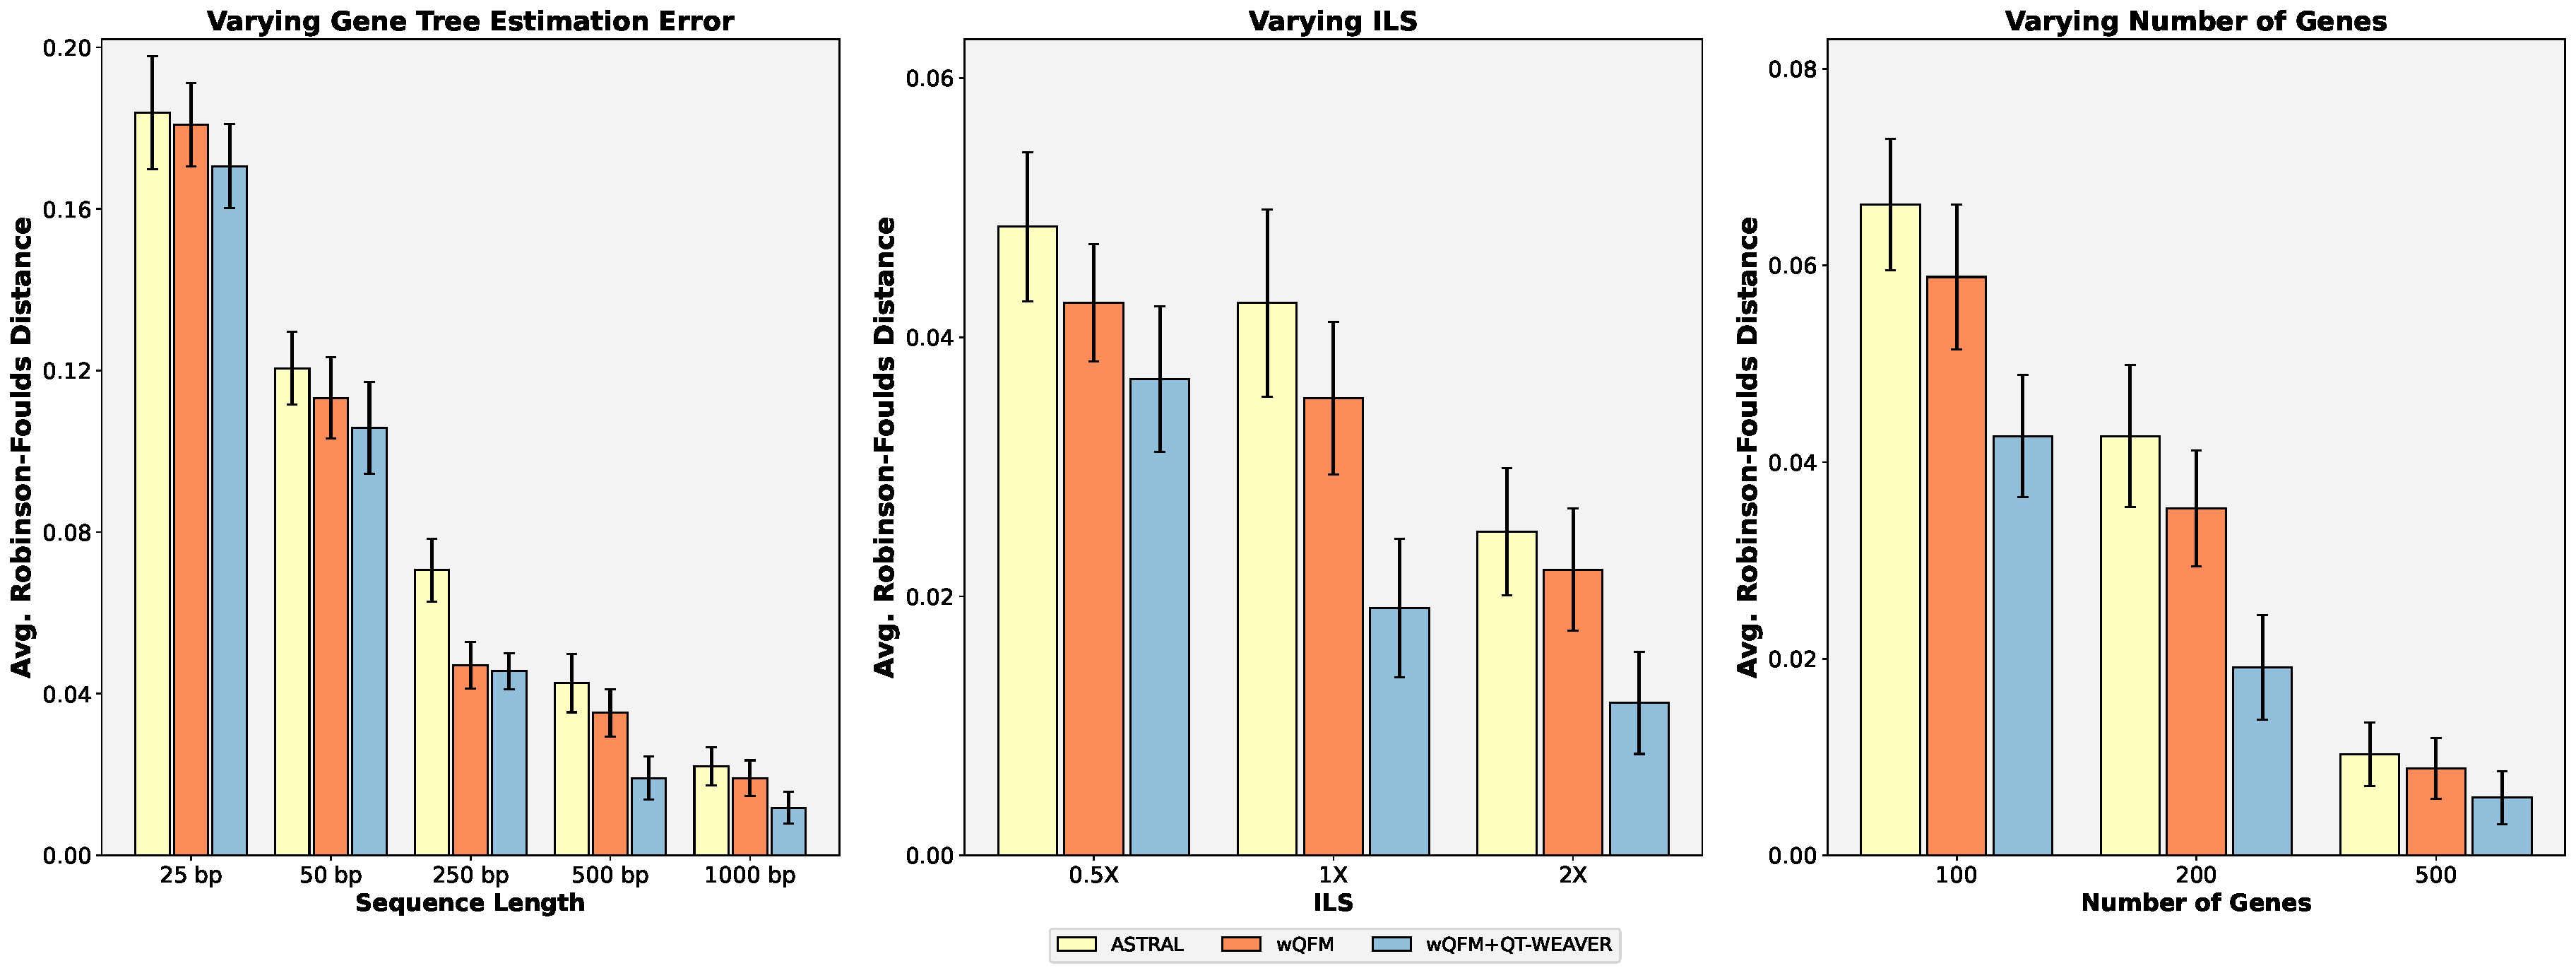
\includegraphics[width=\linewidth]{figures_new/2_37_methods.pdf}
    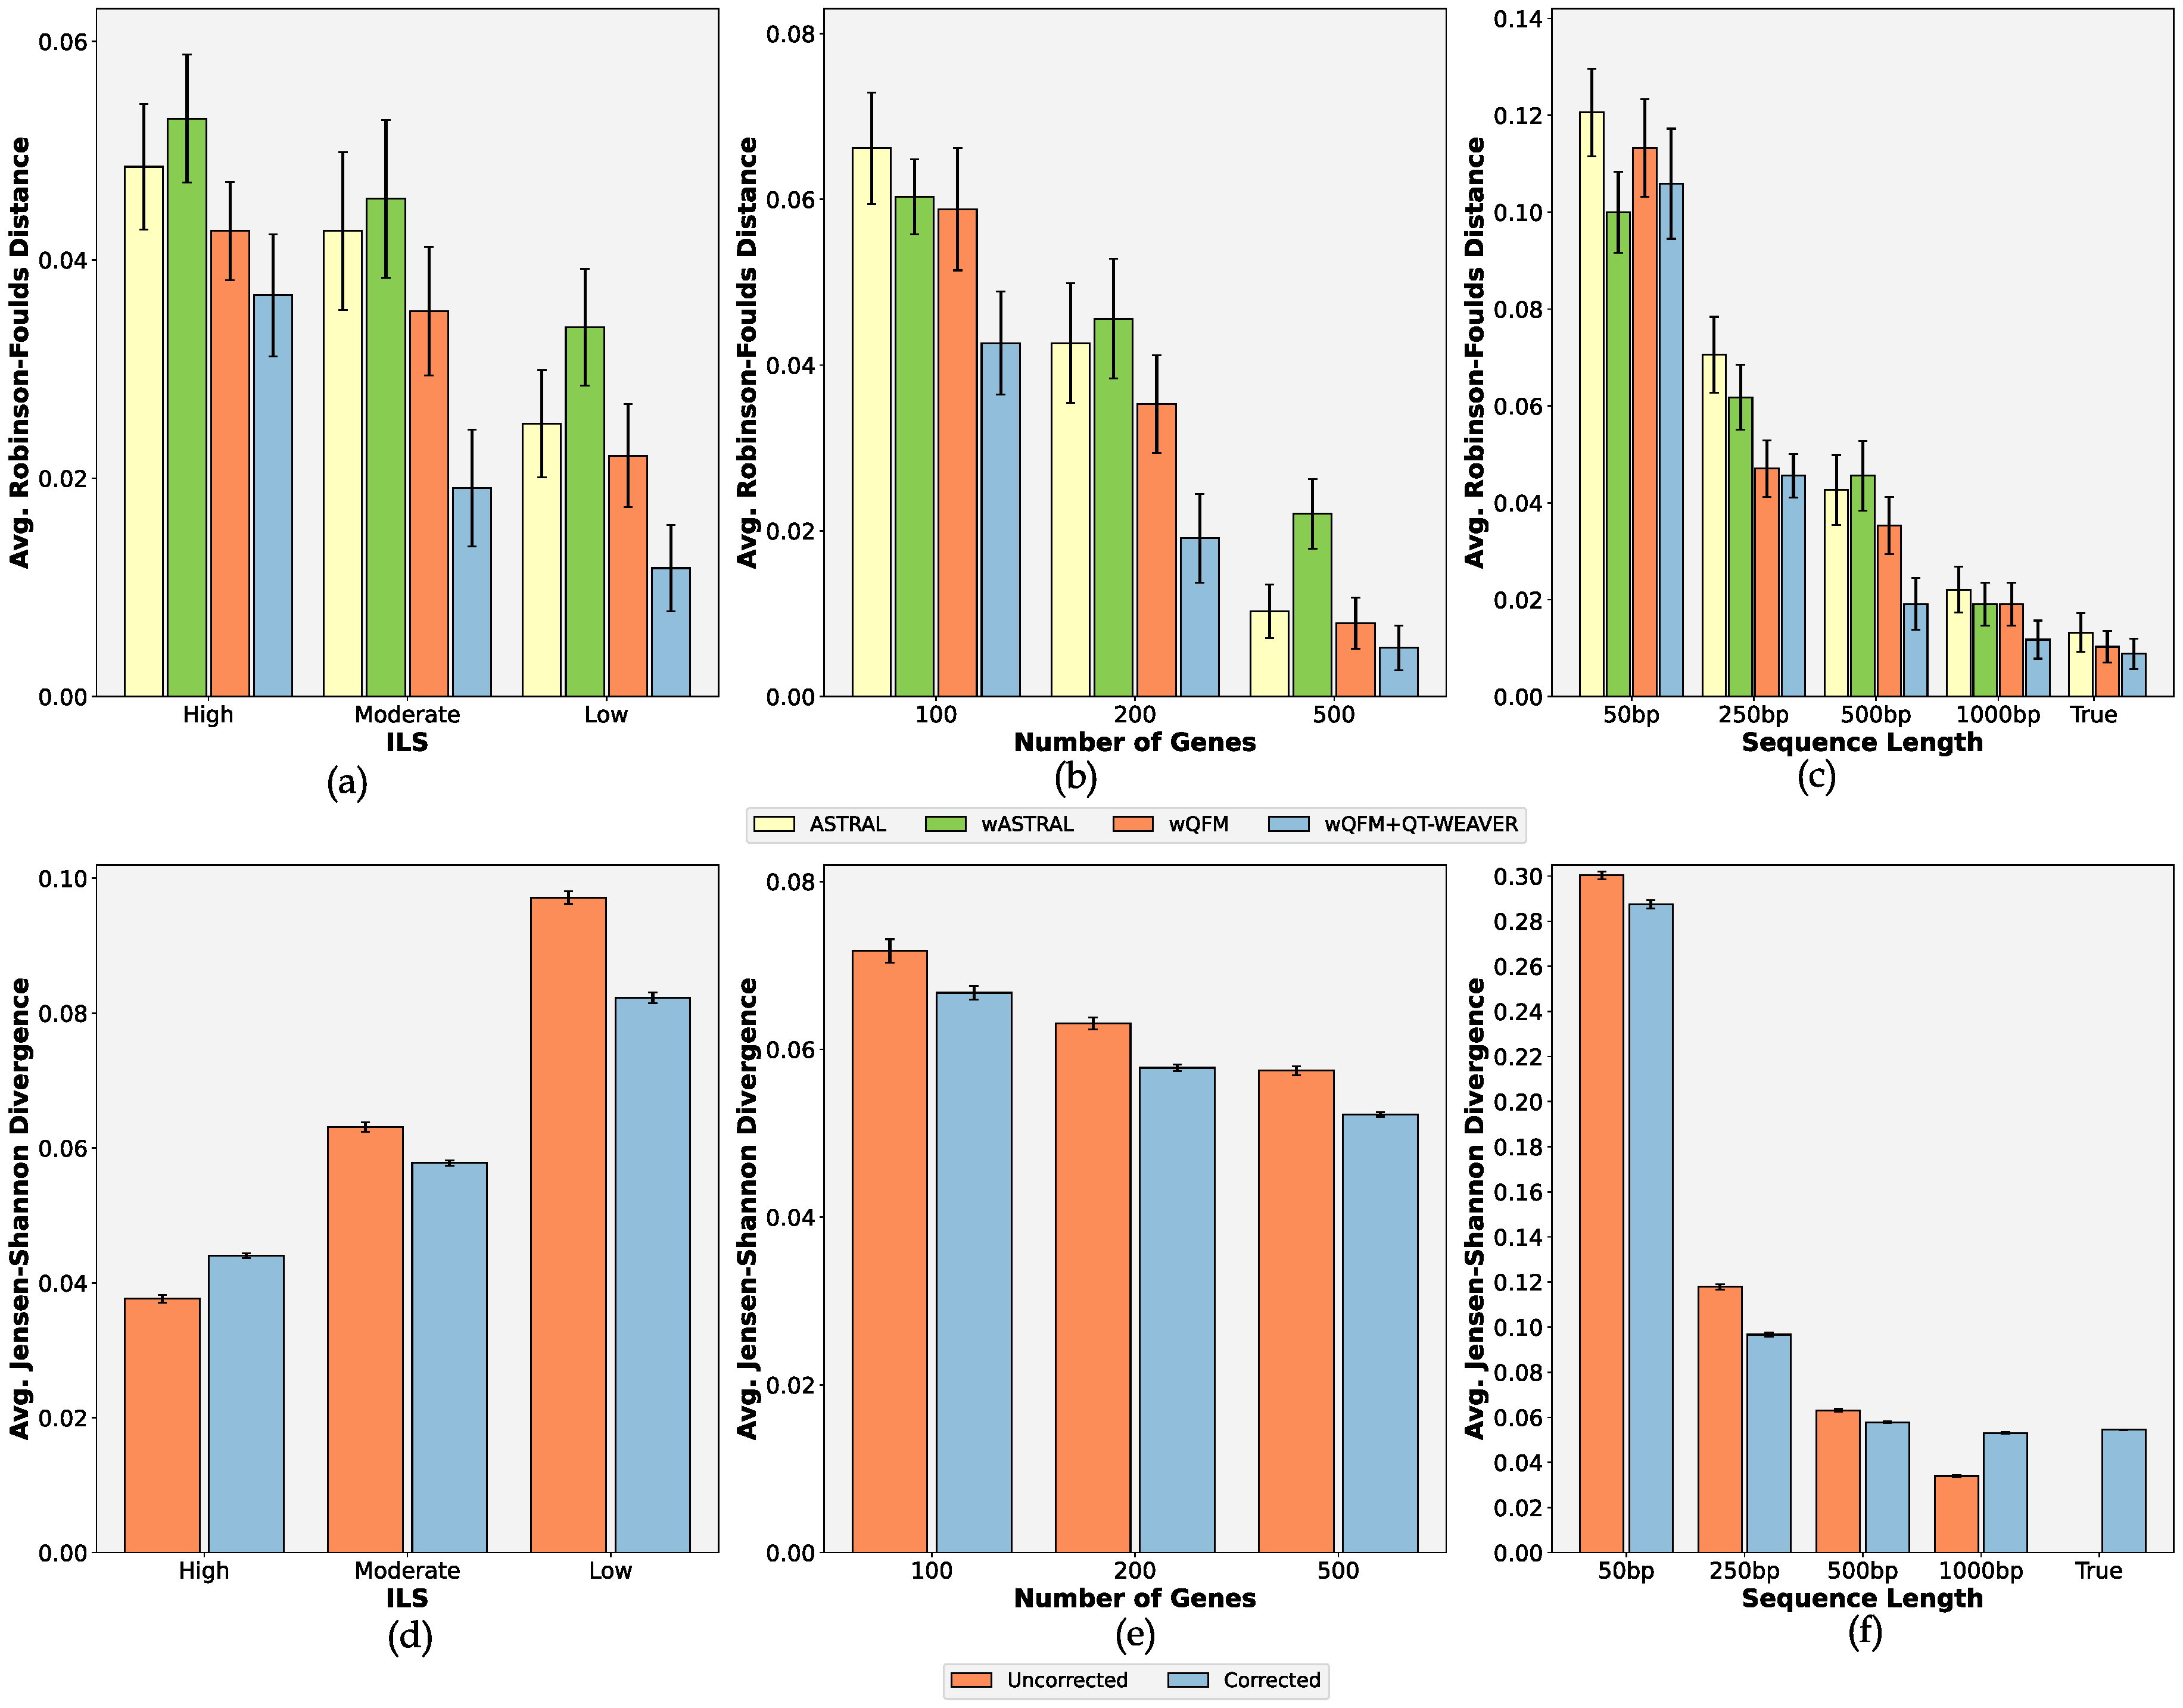
\includegraphics[width=.9\linewidth, height=0.5\linewidth]{figures_new/37-combined-v3.pdf}
    \caption{(a)-(c) Average RF rates with standard errors over 20 replicates for all methods compared. (a) ILS was varied from high to low, keeping the number of genes fixed at 200 and sequence length at 500bp. (b) The number of genes was varied keeping ILS at moderate (1X) and the sequence length at 500bp. (c) Varying sequence lengths with moderate ILS and 200 genes. We also include true gene trees with no GTEE. (d)-(f) Average Jensen-Shannon divergence of the quartet distributions before and after correction with respect to the true quartet distributions. 
    }
    \label{fig:rf_37_taxon_methods}
    \vspace{-10pt}
\end{figure}


\vspace{-10pt}
\subsection{Results on biological avian dataset}
\vspace{-4pt}
%\paragraph{Avian dataset.}
\begin{figure}[h!]  
\centering
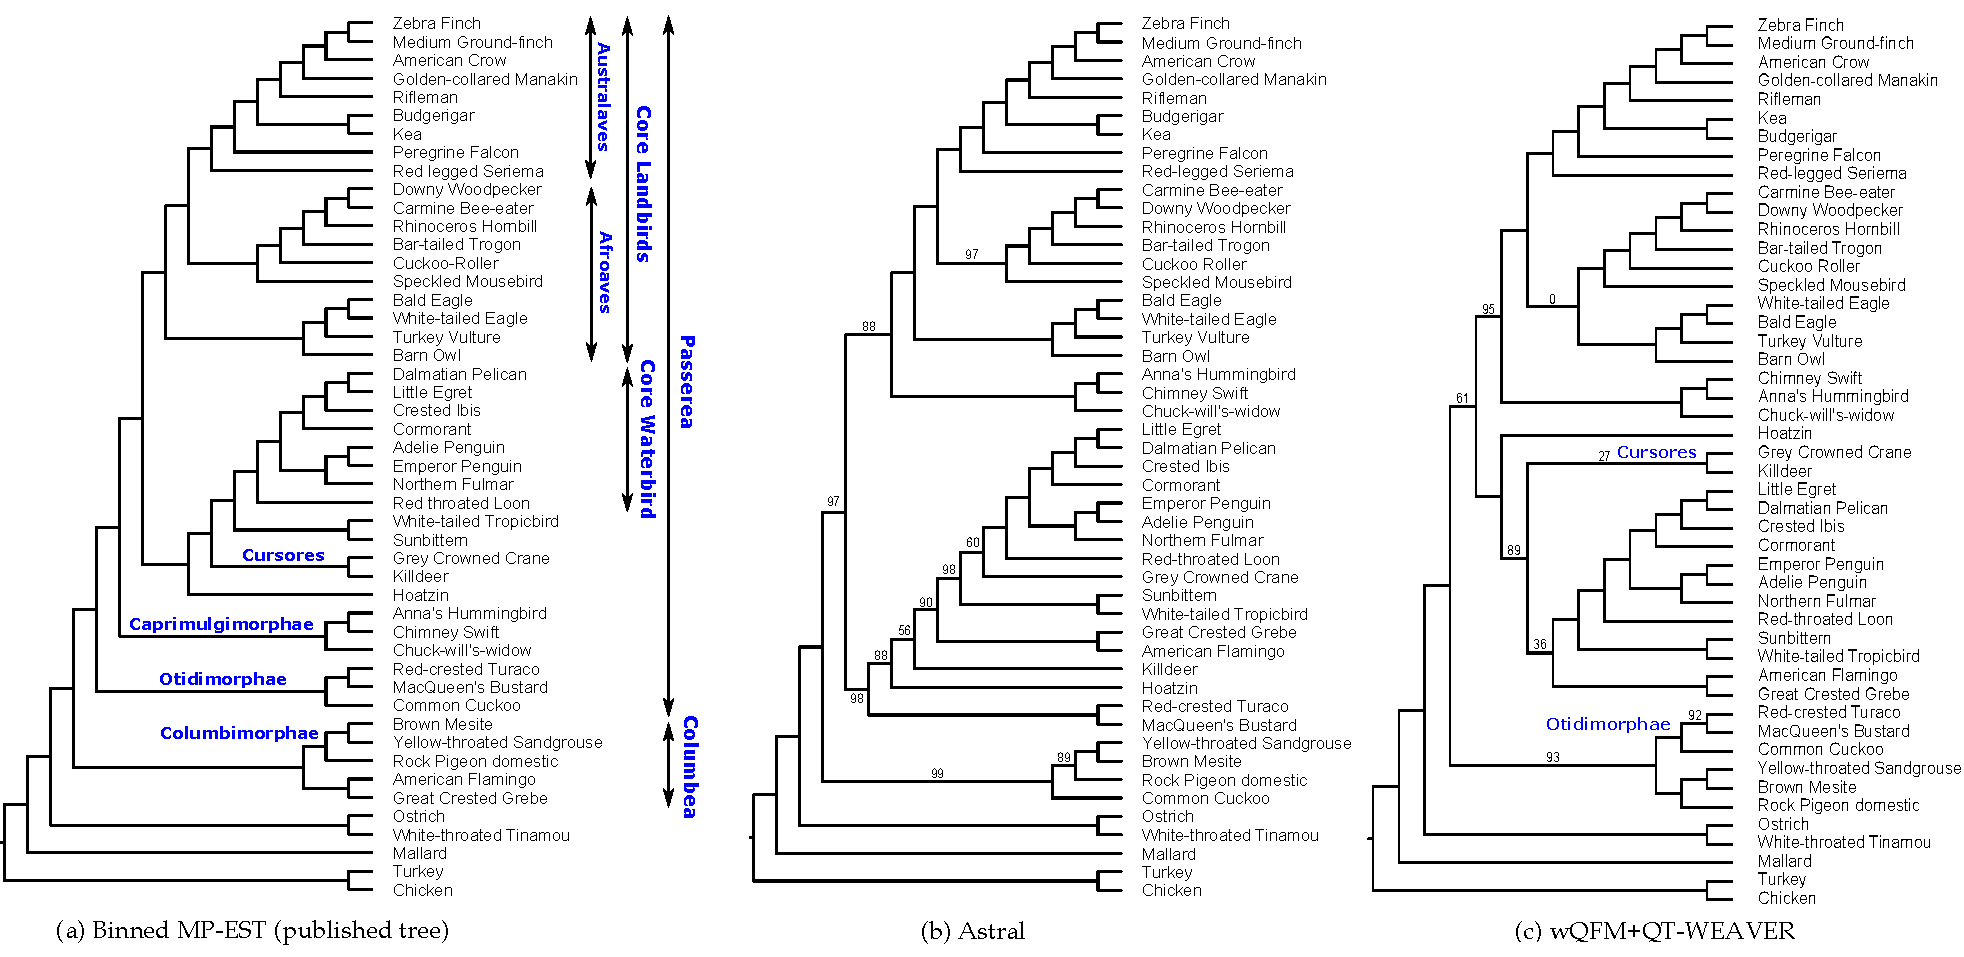
\includegraphics[width=\linewidth, height=0.55\linewidth]{figures_new/avian-trimmed-v2.pdf}
    \caption{Analyses of the avian dataset using binned MP-EST, ASTRAL, and wQFM+QT-WEAVER. 
    Branch supports are computed based on quartet-based local posterior probability~\cite{sayyari2016fast}. All BS values are 100\% except where noted.}
    \label{fig:avian}
\end{figure}

We compare trees estimated by ASTRAL and wQFM+QT-WEAVER in Figure~\ref{fig:avian}. Both trees are highly congruent with the reference binned MP-EST tree presented in~\cite{jarvis2014}, with wQFM+QT-WEAVER being more accurate. ASTRAL failed to recover both the Otidimorphae (bustard,
turaco, and cuckoo) and the Cursores clade (crane and killdeer), both of which wQFM+QT-WEAVER successfully recovered. Both methods successfully reconstructed the well-established Australaves, Afroaves, Core Waterbird, and Caprimulgimorphae clades, but failed to recover Columbea.

\vspace{-10pt}
\section{Conclusions}
\vspace{-8pt}
This study, for the first time, introduces the quartet distribution correction problem and shows the impact and clear benefit of using quartet distributions corrected by QT-WEAVER for improved species tree estimations. %OUr proposed QT-GILD, with its deep autoencoder model with  self-supervision (using masking), effectively learns the underlying quartet distributions and account for gene tree estimation error.
QT-WEAVER learns the overall quartet distribution based on the pattern of quartet conflicts and seeks to update the weights to better reflect their relative importance. Our experimental study shows that QT-WEAVER may result in substantial improvements over the leading method ASTRAL. Moreover, the concept of quartet conflict and related theoretical results have broad applicability and will be valuable for a range of quartet-based computational methods. 
%Our proposed QT-GILD not only imputes the missing quartets but it can also ``correct’’ the estimated quartets -- resulting in a set of quartets that is often closer to the quartet distribution of true gene trees than that of the estimated gene trees, and thereby accounting for gene tree estimation error. Experimental studies using both simulated and real biological dataset suggest that QT-GILD may result in dramatic improvements in species tree accuracy. 
% Therefore, the idea of estimating species trees by correcting quartet distributions has merit and should be pursued and used in future phylogenomic studies. %However, this study can be extended in several directions, especially 
% As a future study, we plan to evaluate QT-WEAVER on a diverse set of real biological datasets as the pattern of quartet conflicts are sufficiently complex and heterogeneous across various datasets. Another important research direction is the automatic selection of QT-WEAVER configurations.
% Additionally, considering the dramatic improvements achieved from multiple iterations of QT-WEAVER on certain datasets and model conditions, future studies need to investigate how to automatically identify an appropriate QT-WEAVER configuration for a given input, based on the input gene tree topologies, to ensure iterative enhancement.
%Because QT-GILD tries to learn the overall quartet distribution guided by a self-supervised feedback loop and correct for gene tree estimation error, investigating its application beyond imputing incomplete gene trees where the goal would be to improve estimated gene tree distributions is another interesting direction to take. In this regard, we can mask a reasonably large number of quartets in the estimated complete quartet distribution and then impute them with QT-GILD, utilizing its error correcting utility. QT-GILD is currently not scalable to large datasets with hundreds of taxa, therefore this study was limited to small to moderate size datasets. Future study needs to develop a scalable variant of QT-GILD and assess its performance on large dataset.


% for extended version (journal version): add scalability issue. also generalizability issue. it may not work well on some dataset. More extensive evaluation studies.








%
% ---- Bibliography ----
%
% BibTeX users should specify bibliography style 'splncs04'.
% References will then be sorted and formatted in the correct style.
%
\bibliographystyle{splncs04}
\bibliography{references.bib} 

%
% \begin{thebibliography}{8}
% \bibitem{ref_article1}
% Author, F.: Article title. Journal \textbf{2}(5), 99--110 (2016)

% \bibitem{ref_lncs1}
% Author, F., Author, S.: Title of a proceedings paper. In: Editor,
% F., Editor, S. (eds.) CONFERENCE 2016, LNCS, vol. 9999, pp. 1--13.
% Springer, Heidelberg (2016). \doi{10.10007/1234567890}

% \bibitem{ref_book1}
% Author, F., Author, S., Author, T.: Book title. 2nd edn. Publisher,
% Location (1999)

% \bibitem{ref_proc1}
% Author, A.-B.: Contribution title. In: 9th International Proceedings
% on Proceedings, pp. 1--2. Publisher, Location (2010)

% \bibitem{ref_url1}
% LNCS Homepage, \url{http://www.springer.com/lncs}, last accessed 2023/10/25
% \end{thebibliography}



\end{document}
